\begin{figure}[tbp]
\centering
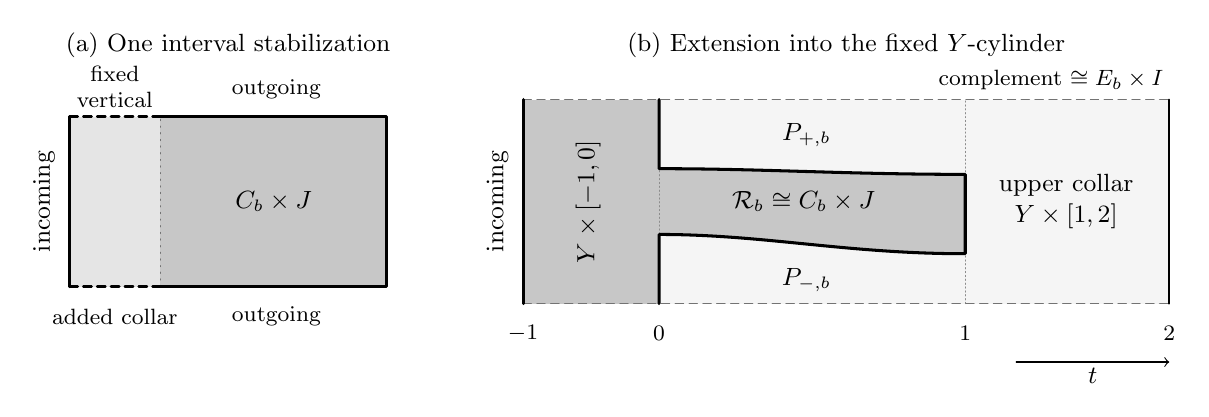
\begin{tikzpicture}[x=0.72cm,y=0.72cm,font=\small,
  every node/.style={inner sep=2pt},line cap=round,line join=round]
  \node at (2.8,5.25) {(a) One interval stabilization};
  \fill[black!10] (0,1) rectangle (1.6,4);
  \fill[black!22] (1.6,1) rectangle (5.6,4);
  \draw[line width=1.1pt] (0,1)--(0,4);
  \draw[densely dashed,line width=0.9pt] (0,1)--(1.6,1);
  \draw[densely dashed,line width=0.9pt] (0,4)--(1.6,4);
  \draw[black!55,dotted] (1.6,1)--(1.6,4);
  \draw[line width=1.1pt] (1.6,1)--(5.6,1)--(5.6,4)--(1.6,4);
  \node[rotate=90] at (-0.45,2.5) {incoming};
  \node at (3.6,2.5) {$C_b\times J$};
  \node[align=center,font=\footnotesize] at (0.8,4.53)
    {fixed\\vertical};
  \node[font=\footnotesize] at (3.65,4.48) {outgoing};
  \node[align=center,font=\footnotesize] at (0.8,0.47)
    {added collar};
  \node[font=\footnotesize] at (3.65,0.47) {outgoing};

  \node at (13.7,5.25) {(b) Extension into the fixed $Y$-cylinder};
  \fill[black!4] (8,0.7) rectangle (19.4,4.3);
  \fill[black!22] (8,0.7) rectangle (10.4,4.3);
  \path[fill=black!22]
    (10.4,1.92) .. controls (12.25,1.92) and (13.7,1.58) .. (15.8,1.58)
    --(15.8,2.98) .. controls (13.7,2.98) and (12.25,3.08) .. (10.4,3.08)
    --cycle;
  \draw[black!45,densely dotted] (10.4,0.7)--(10.4,4.3);
  \draw[black!45,densely dotted] (15.8,0.7)--(15.8,4.3);
  \draw[black!55,densely dashed] (8,0.7)--(19.4,0.7);
  \draw[black!55,densely dashed] (8,4.3)--(19.4,4.3);
  \draw[line width=1.1pt] (8,0.7)--(8,4.3);
  \draw[line width=0.7pt] (19.4,0.7)--(19.4,4.3);
  \draw[line width=1.1pt]
    (10.4,0.7)--(10.4,1.92)
    .. controls (12.25,1.92) and (13.7,1.58) .. (15.8,1.58)
    --(15.8,2.98)
    .. controls (13.7,2.98) and (12.25,3.08) .. (10.4,3.08)
    --(10.4,4.3);
  \node[rotate=90] at (7.55,2.5) {incoming};
  \node[rotate=90] at (9.15,2.5) {$Y\times[-1,0]$};
  \node at (12.95,2.5) {$\mathcal R_b\cong C_b\times J$};
  \node at (13.0,3.68) {$P_{+,b}$};
  \node at (13.0,1.12) {$P_{-,b}$};
  \node[align=center] at (17.58,2.5) {upper collar\\$Y\times[1,2]$};
  \node[anchor=east,font=\footnotesize] at (19.4,4.65)
    {complement $\cong E_b\times I$};
  \node[font=\footnotesize] at (10.4,0.18) {$0$};
  \node[font=\footnotesize] at (8,0.18) {$-1$};
  \node[font=\footnotesize] at (15.8,0.18) {$1$};
  \node[font=\footnotesize] at (19.4,0.18) {$2$};
  \draw[->,thin] (16.7,-0.33)--(19.4,-0.33)
    node[midway,below] {$t$};
\end{tikzpicture}
\caption{Face bookkeeping for one fiber, before corner rounding.
In (a), the dashed segments are the fixed vertical faces on the added
incoming collar $\Sigma\times[-1,0]\times J$; both sides beyond that
collar are movable outgoing faces. In (b), the dark region is
$W_b=(Y\times[-1,0])\cup\mathcal R_b$, and its heavy interface with
the light complement is $E_b=\partial_+W_b$. The product identification
of the complement is proved over the possibly varying bundle $E\to B$.
The angular direction is schematic: the upper and lower dashed display
edges are not boundary faces of the closed sphere $Y$. The drawing
asserts neither radial monotonicity nor a product trivialization of
$C\to B$.}
\label{fig:regular-band}
\end{figure}
